%%%%%%%%%%%%%%%%%%%%%%%%%%%%%%%%%%%%%%%%%%%%%%%%%%%%%%%%%%%%
%%% LaPreprint: PREPRINT TEMPLATE
%%%%%%%%%%%%%%%%%%%%%%%%%%%%%%%%%%%%%%%%%%%%%%%%%%%%%%%%%%%%

% Here I could talk about what one should do in this document.
% Instead I'll refer you to the explore on your own and check the Github Repo. :-)
% Line spacing is 1.2 by default (can't be smaller).

%%%%%%%%%%%%%%%%%%%%%%%%%%%%%%%%%%%%%%%%%%%%%%%%%%%%%%%%%%%%
%%% PREAMBLE
%%%%%%%%%%%%%%%%%%%%%%%%%%%%%%%%%%%%%%%%%%%%%%%%%%%%%%%%%%%%

% Declare document class
\documentclass[9pt,biorxiv,lineno]{lapreprint}
% Choose between "biorxiv", "medrxiv", "arxiv" and "chemrxiv". Otherwise defaults "Preprint".
% Choose between "blue" and "red" colour scheme. Defaults to "blue".
% Use the "onehalfspacing" option for 1.5 line spacing.
% Use the "doublespacing" option for 2.0 line spacing.
% Use the "lineno" option for line numbers.
% Use the "endfloat" option to place floats after the bibliography.
% Use the "secnum" option to have include numbers.

% Import packages
% \usepackage{lipsum}     % Required to insert dummy text
\usepackage[version=4]{mhchem} % For chemical notation
\usepackage{siunitx}    % For SI units
\usepackage{pdflscape}  % For putting pages in landscape mode
\usepackage{rotating}   % For rotating specific elements
\usepackage{textgreek}  % Greek symbols
\usepackage{gensymb}    % Symbols
\usepackage[misc]{ifsym} % For the \Letter symbol
\usepackage{orcidlink}  % For the \orcidlink
\usepackage{listings}   % For inserting code chunks
\usepackage{colortbl}   % For Knitr table colouring
\usepackage{tabularx}   % For making Knitr tables compatible
\usepackage{longtable}  % For multi-page tables
\usepackage{subcaption}
\usepackage{multirow}
\usepackage{snotez}     % For sidenote environments. enotez for endnotes
\usepackage{csquotes}   % For language-based quote rules (helps BiBLaTeX)

% Make declarations
\DeclareSIUnit\Molar{M}

% Please note that these options may affect formatting. 

%%%%%%%%%%%%%%%%%%%%%%%%%%%%%%%%%%%%%%%%%%%%%%%%%%%%%%%%%%%%
%%% BIBLIOGRAPHY
%%%%%%%%%%%%%%%%%%%%%%%%%%%%%%%%%%%%%%%%%%%%%%%%%%%%%%%%%%%%
\usepackage[			% use biblatex for bibliography
	backend=biber,      % use biber or bibtex backend
    style=authoryear,   % choose style
	natbib=true,		% allow natbib commands
	hyperref=true,	    % activate hyperref support
	alldates=year,      % only show year (not month)
    uniquename=false,   % don't add firstnames when citing multiple sources by the same author
    maxbibnames=99,     % maximum number of author names to list in bibliography before 'et al' is used instead
]{biblatex}

% Just avoiding some rogue fields that cause issues with certain styles 
\AtEveryBibitem{
    \clearfield{urlyear}
    \clearfield{urlmonth}
    \clearlist{language}
}

% Update to your bibliography file
\addbibresource{src/bibliography.bib}

%%%%%%%%%%%%%%%%%%%%%%%%%%%%%%%%%%%%%%%%%%%%%%%%%%%%%%%%%%%%
%%% ARTICLE SETUP
%%%%%%%%%%%%%%%%%%%%%%%%%%%%%%%%%%%%%%%%%%%%%%%%%%%%%%%%%%%%

% Paper title
\title{LaPreprint: \\ A Preprint Template for \LaTeX}

% Authors - you can use \orcidlink{} and \authfn{} - see contribution note
\author[ \orcidlink{0000-0002-9998-0058} 1 \Letter]{Mikkel Roald-Arb\o l}
\author[2]{Co-author}

% Affiliations
\affil[1]{School of Life Sciences, University of Sussex}
\affil[2]{University of Somewhere}

% Other metadata. Feel free to add your own
\metadata[]{\Letter\hspace{.5ex} For correspondence}{\url{https://github.com/roaldarbol/LaPreprint/issues} (MRA)}
\metadata[\authfn{1}\authfn{2}\authfn{3}]{}{Here's a few symbols to denote contribution specifics, e.g. authors who contributed equally to the work.}
\metadata[]{Present address}{Evolution, Behaviour and Environment, School of Life Sciences, University of Sussex, Biology Road, Brighton, BN1 9RH, United Kingdom}
\metadata[]{Data availability}{Data availability statement. Preprocessed data could be available e.g. on \href{https://zenodo.org/}{Zenodo}.}
\metadata[]{Funding}{MRA was supported by funding from the Leverhulme Foundation. The funders had no role in the template design or decision to publish.}
\metadata[]{Competing interests}{The author declare no competing interests.}


% Surname of the lead author(s) for the running footer
\leadauthor{Roald-Arb\o l}
\shorttitle{A Preprint Template for \LaTeX}

%%%%%%%%%%%%%%%%%%%%%%%%%%%%%%%%%%%%%%%%%%%%%%%%%%%%%%%%%%%%
%%% ARTICLE START
%%%%%%%%%%%%%%%%%%%%%%%%%%%%%%%%%%%%%%%%%%%%%%%%%%%%%%%%%%%%

\begin{document}
\maketitle
\begin{abstract}

Let's begin with some great papers for those interested in radically improving the scientific infrastructure \parencite{Pooley2021, Bezuidenhout2021,Brembs2021}. \lipsum[1]

\end{abstract}
\section{Introduction} \label{intro}
Use \verb|\section| and \verb|\subsection| commands to organize your document. \LaTeX{} handles all the formatting automatically. Use \verb|\label| and \verb|\nameref| commands for cross-referencing sectional headings: the usual \verb|\ref| will not work, as this template uses unnumbered sectional headings. \par
\lipsum[2]

\subsection{Figures and Tables}
Use the table and tabular commands for basic tables --- see \TABLE{example}, for example. For tables, I recommend that you use a separate .tex file for each table and insert it using \verb|\input{mytable.tex}|.

You can upload a figure (JPEG, PNG or PDF) using the project menu. To include it in your document, use the \verb|\includegraphics| command as in the code for \FIG{view}. 

Really wide figures or tables, that take up the entire page, including the gutter space: use \verb|\begin{fullwidth}...\end{fullwidth}| as in \FIG{fullwidth}. And sometimes you may want to use feature boxes like \BOX{simple}.

\begin{figure}
    \begin{fullwidth}
    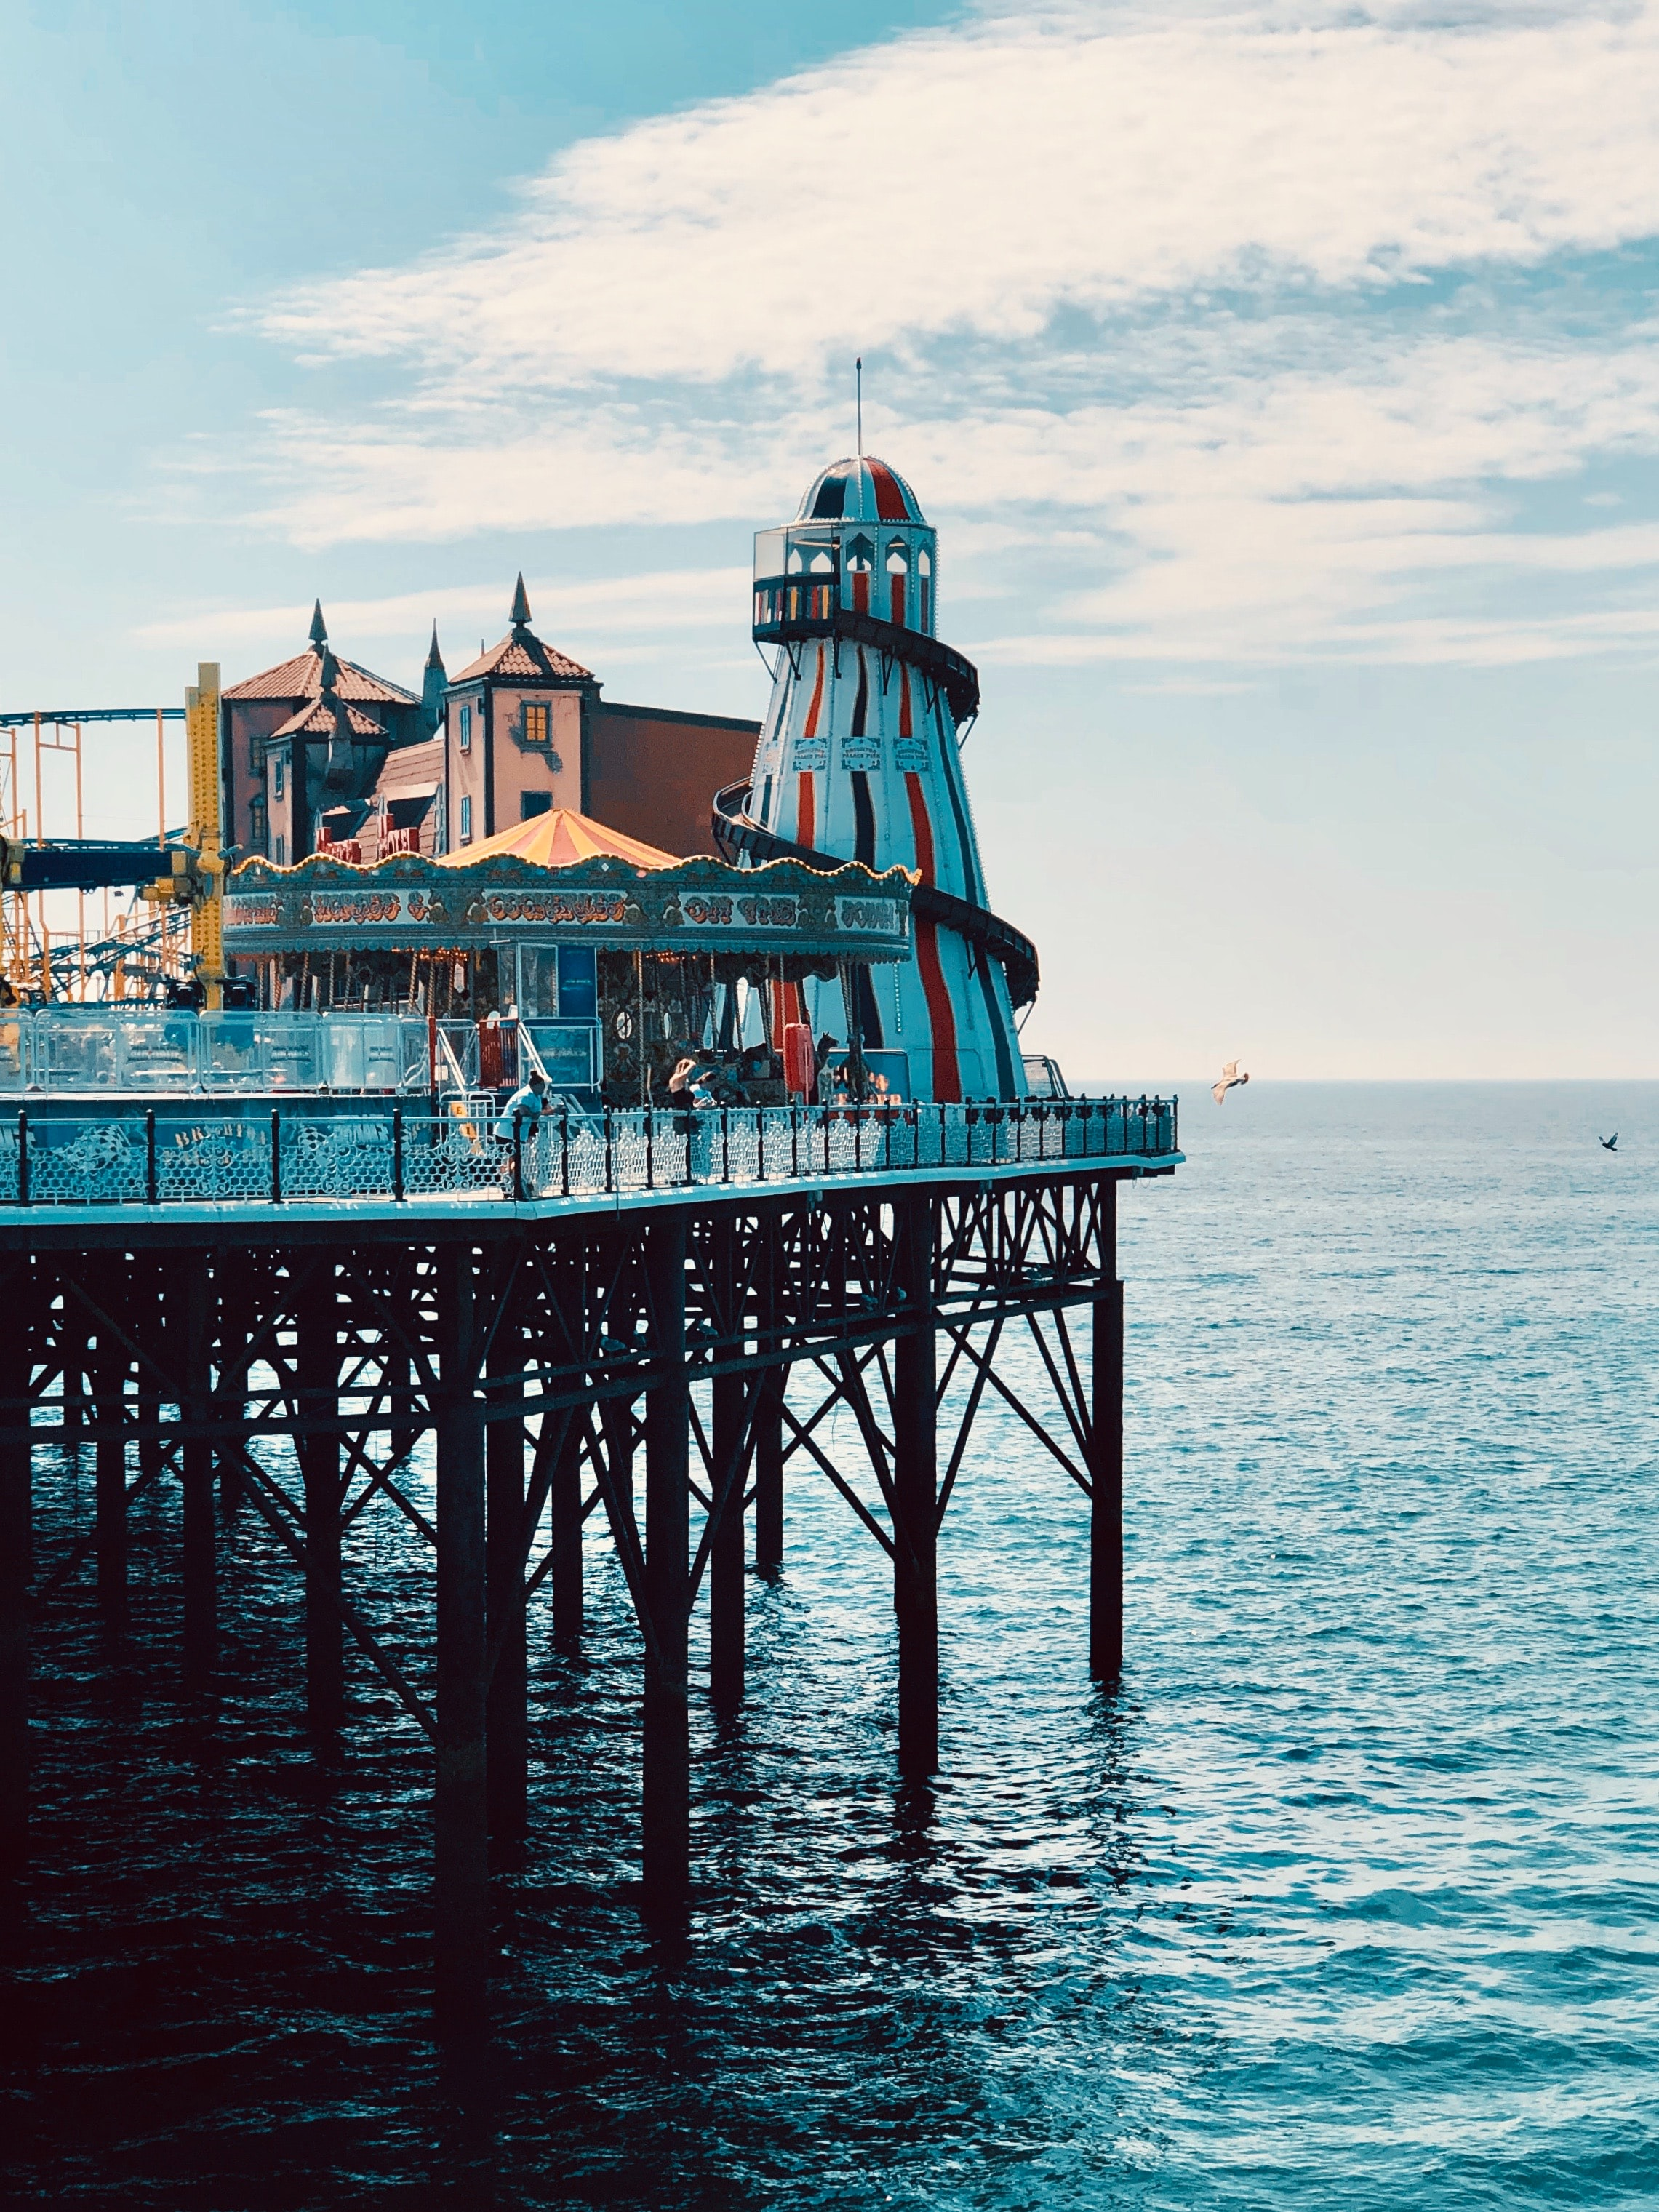
\includegraphics[width=0.65\textheight]{src/figures/brighton.jpeg}
    \caption{\textbf{Photo of lovely Brighton by \href{https://unsplash.com/es/@sanekovs?utm_source=unsplash&utm_medium=referral&utm_content=creditCopyText"}{Alex Ovs} on \href{https://unsplash.com/s/photos/brighton?utm_source=unsplash&utm_medium=referral&utm_content=creditCopyText}{Unsplash}.
    } As a very wide figure that takes up the entire page, including the gutter space.}
    \label{fig:fullwidth}
    \figsupp{There is no limit on the number of Figure Supplements for any one primary figure. Each figure supplement should be clearly labelled, Figure 1--Figure Supplement 1, Figure 1--Figure Supplement 2, Figure 2--Figure Supplement 1 and so on, and have a short title (and optional legend). Figure Supplements should be referred to in the legend of the associated primary figure, and should also be listed at the end of the article text file.}{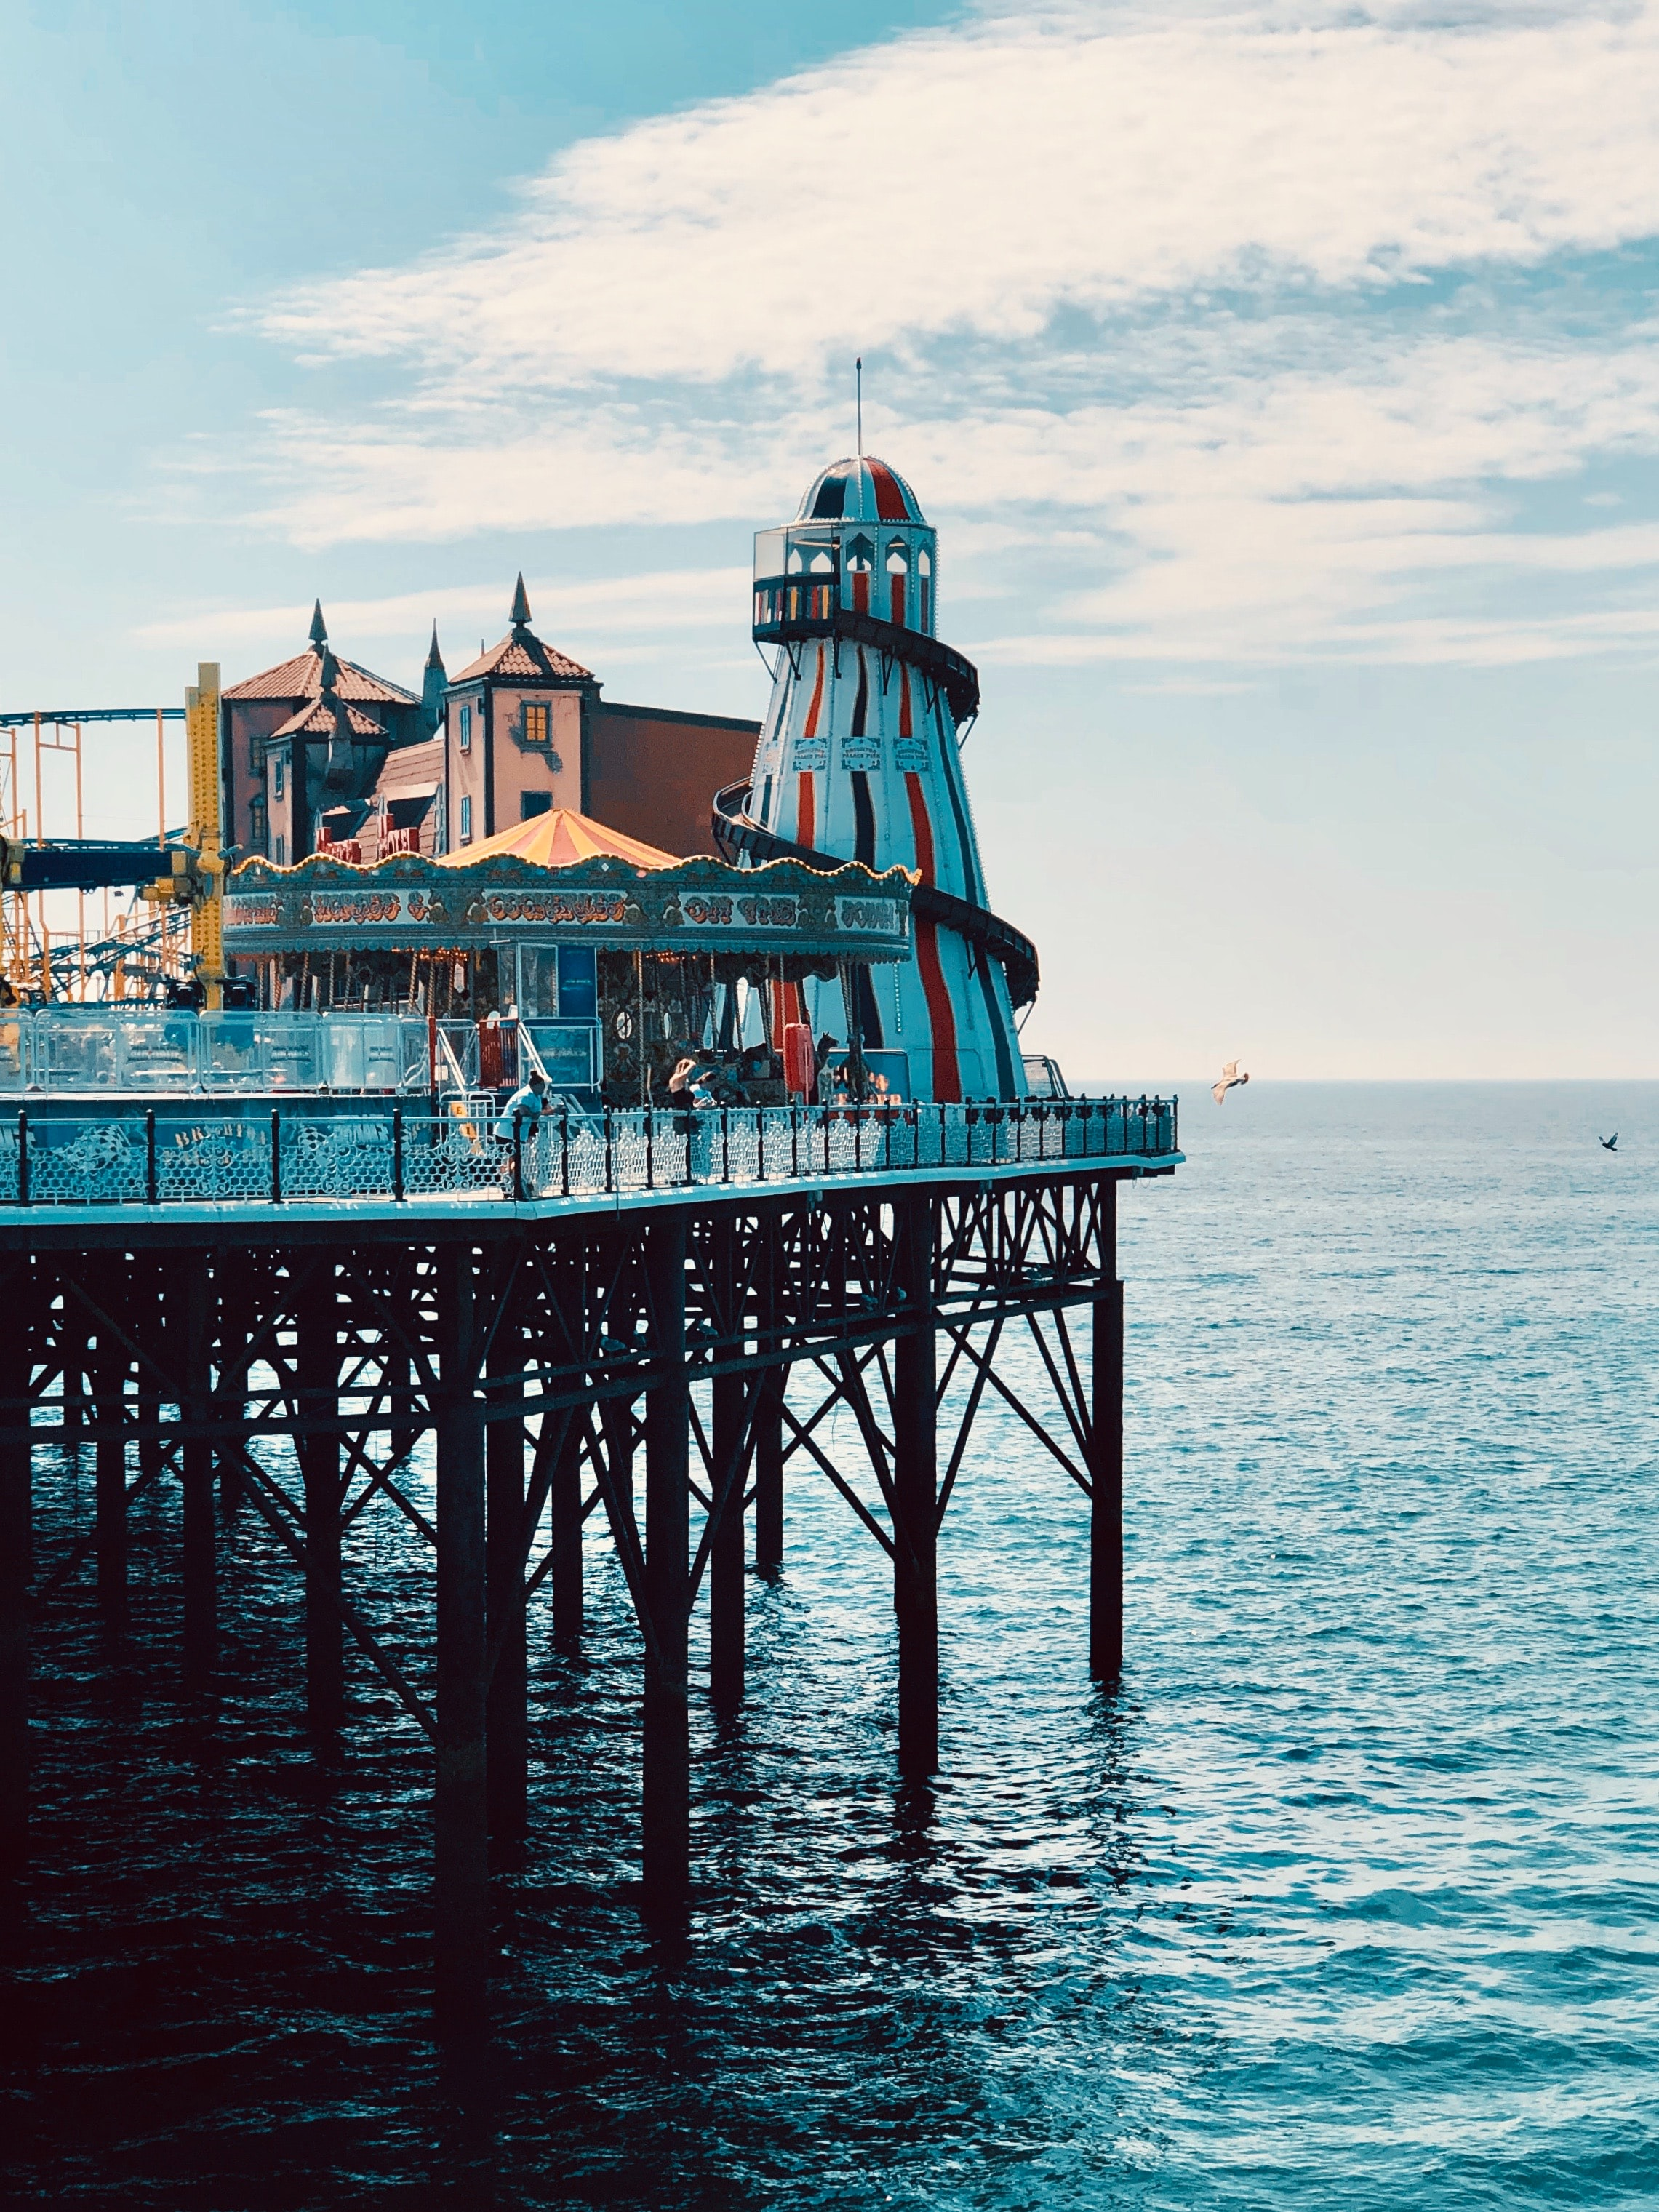
\includegraphics[width=5cm]{src/figures/brighton.jpeg}}
    \end{fullwidth}
\end{figure}

\subsection{Citations and notes}

LaTeX formats citations and references automatically using the bibliography records in your .bib file. Use the \verb|\cite| command for an inline citation, like \cite{Pooley2021}, and the \verb|\parencite| command for a citation in parentheses \parencite{Brembs2021}. Side notes makes good use of the empty margin and can be used ewith the \verb|\sidenote| command. \sidenote{This is a sidenote made with the \textbackslash sidenote package. \lipsum[1]}


\begin{featurebox}
\caption{This is an example feature box}
\label{box:simple}
This is a feature box. It floats!
\medskip

\includegraphics[width=5cm]{example-image}
\featurefig{`Figure' and `table' captions in feature boxes should be entered with \texttt{\textbackslash featurefig} and \texttt{\textbackslash featuretable}. They're not really floats.}

\lipsum[1]
\end{featurebox}

\subsection{Mathematics}

\LaTeX{} is great at typesetting mathematics $abc$. Let $X_1, X_2, \ldots, X_n$ be a sequence of independent and identically distributed random variables with $\text{E}[X_i] = \mu$ and $\text{Var}[X_i] = \sigma^2 < \infty$, and let
\begin{equation}
\label{eq:CLT}
S_n = \frac{X_1 + X_2 + \cdots + X_n}{n}
      = \frac{1}{n}\sum_{i}^{n} X_i
\end{equation}
denote their mean. Then as $n$ approaches infinity, the random variables $\sqrt{n}(S_n - \mu)$ converge in distribution to a normal $\mathcal{N}(0, \sigma^2)$.

You can even get extra fancy and annotate your equations directly: %this uses the `annotate-equations` package. See `https://ctan.org/pkg/annotate-equations` for further info and ideas

\vspace{1.5em} 
\begin{equation}
\label{eq:CLT2}
S_n = \frac{\eqnmarkbox[blue]{a1}{X_1 + X_2 + \cdots + X_n}}{n}
      = \frac{1}{n}\sum_{i}^{n} \eqnmarkbox[purple]{a2}{X_i}
\end{equation}
\annotate[yshift=1em]{above}{a1}{independent and identically distributed random variables}
\annotate[yshift=-1em]{below,left}{a2}{a random variable}
\vspace{1.5em} 

\lipsum[3] 

\begin{figure}
    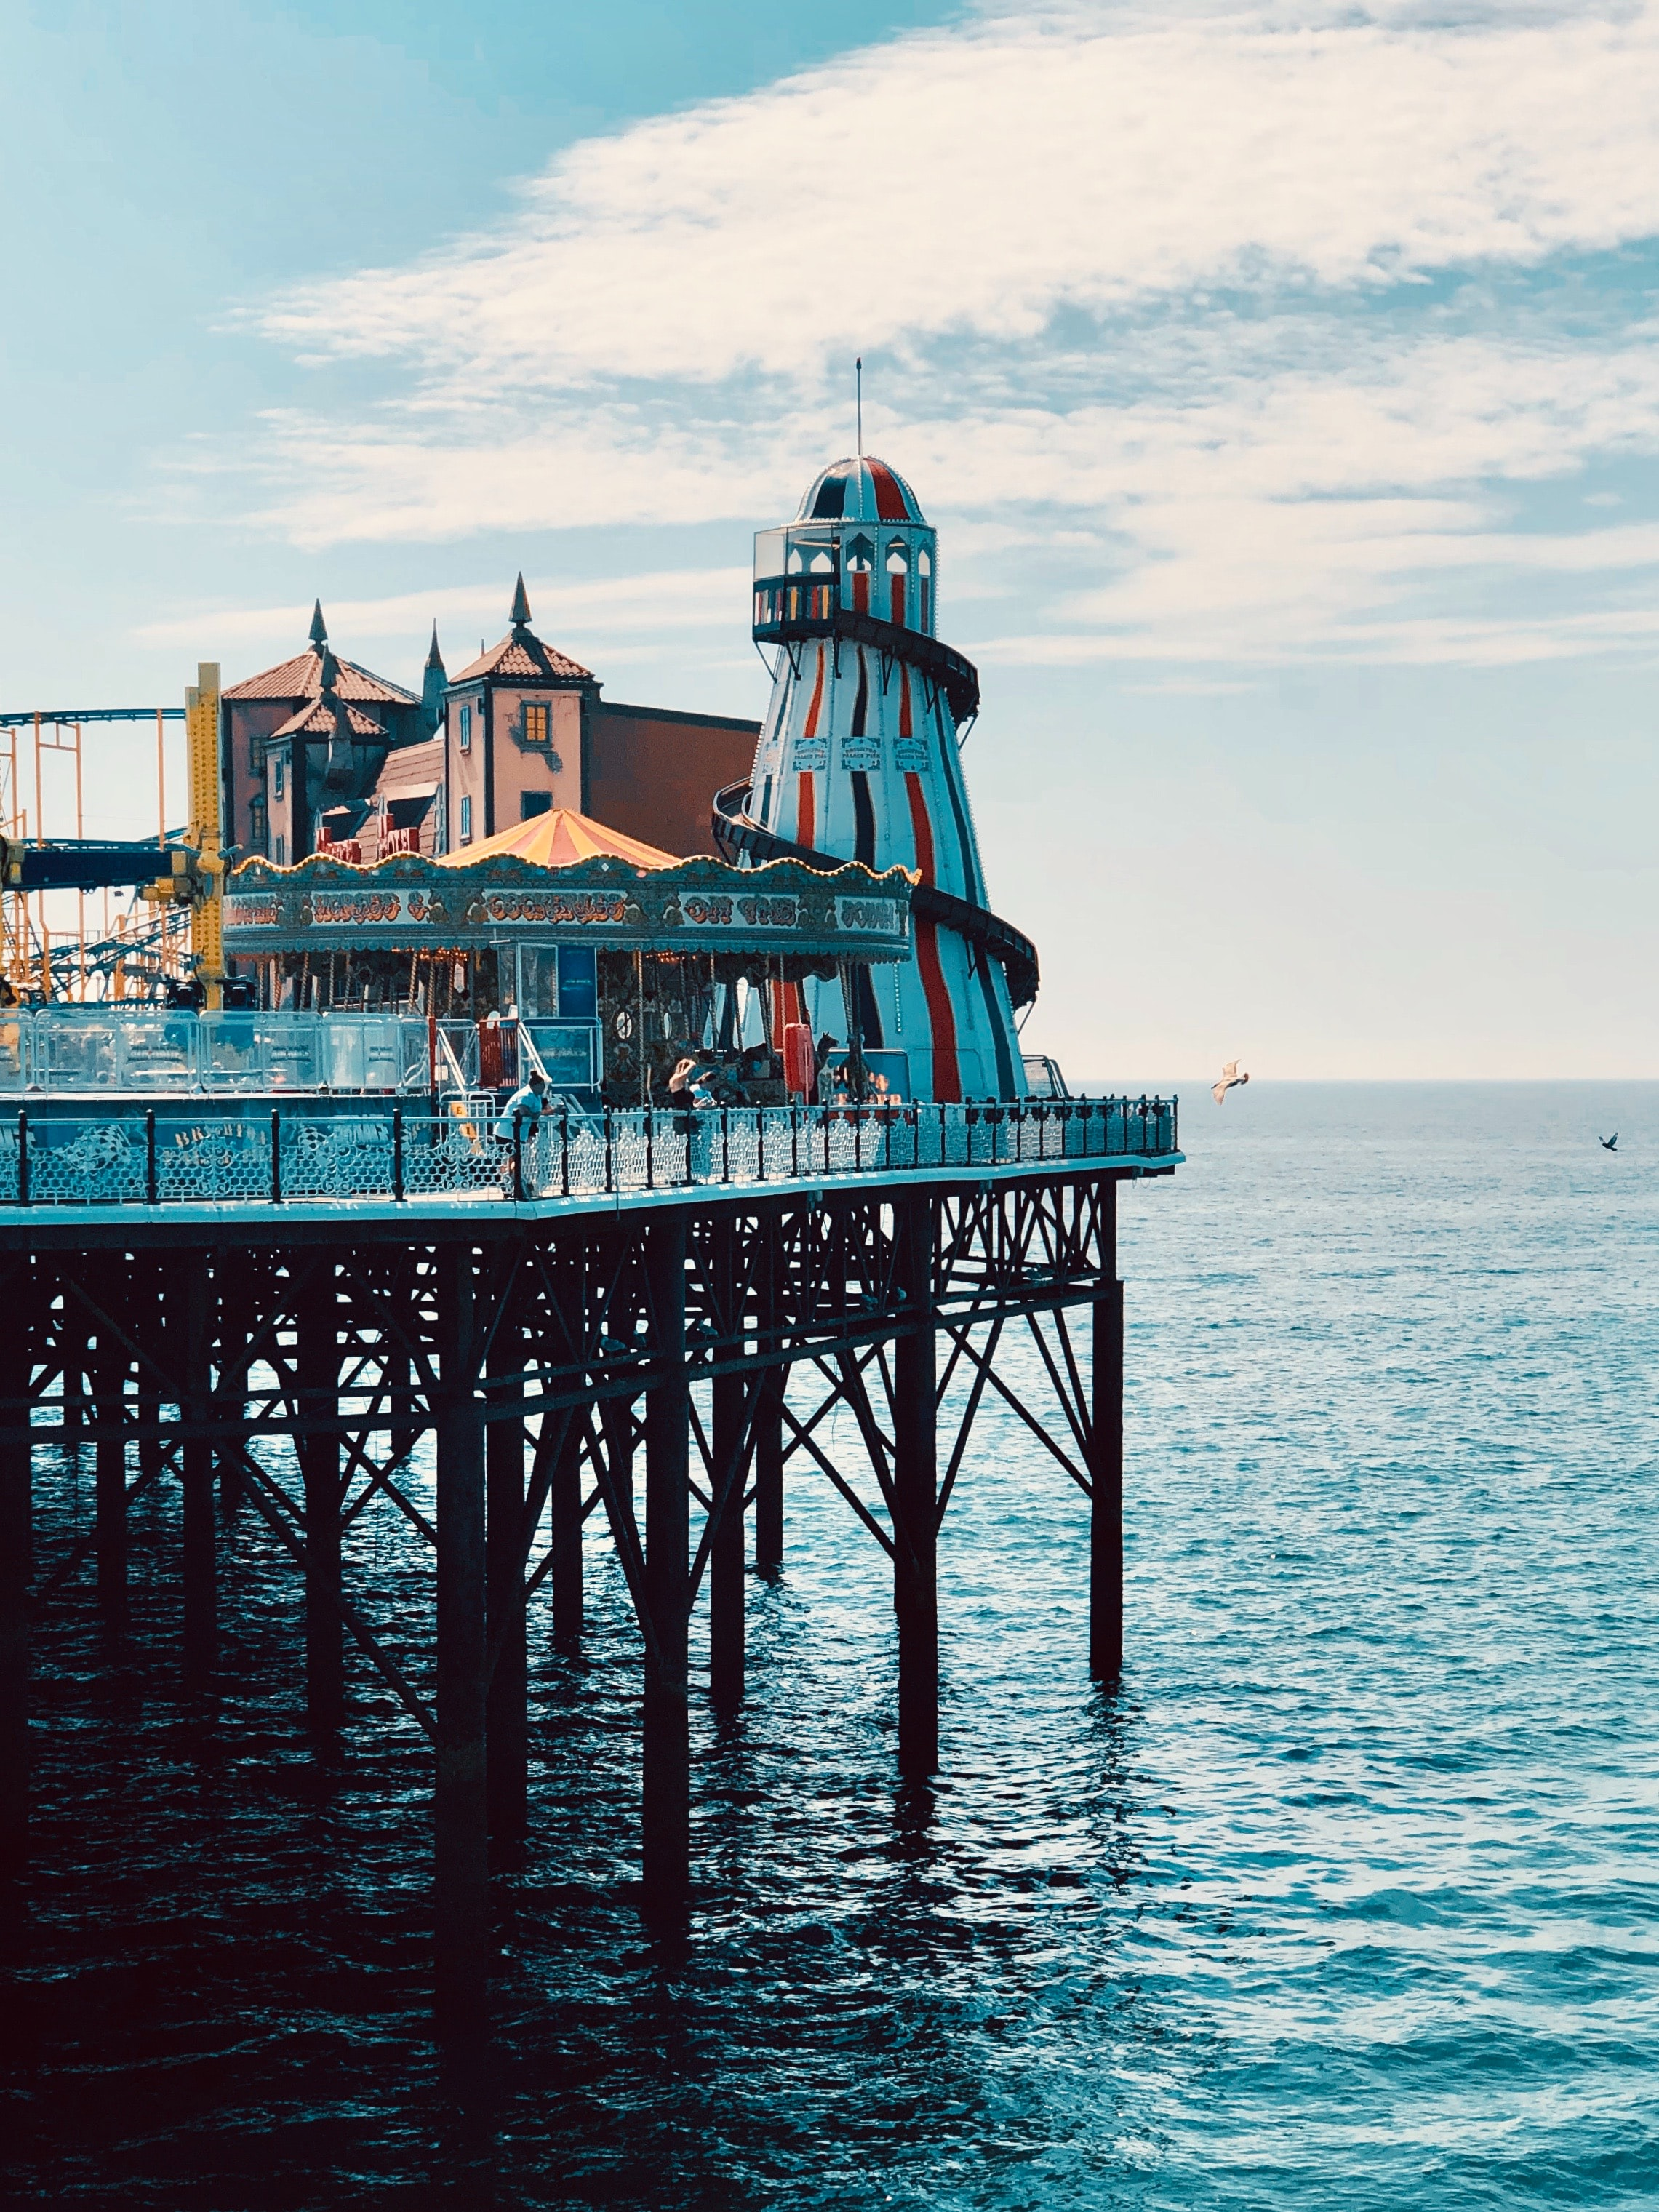
\includegraphics[width=\linewidth]{src/figures/brighton.jpeg}
    \caption{A text-width example.}
    \label{fig:view}
    %% If the optional argument in the square brackets is "none", then the caption *will not appear in the main figure at all* and only the full caption will appear under the supplementary figure at the end of the manuscript.
    \figsupp[Shorter caption for main text.]{This is a supplementary figure's full caption, which will be used at the end of the manuscript.}{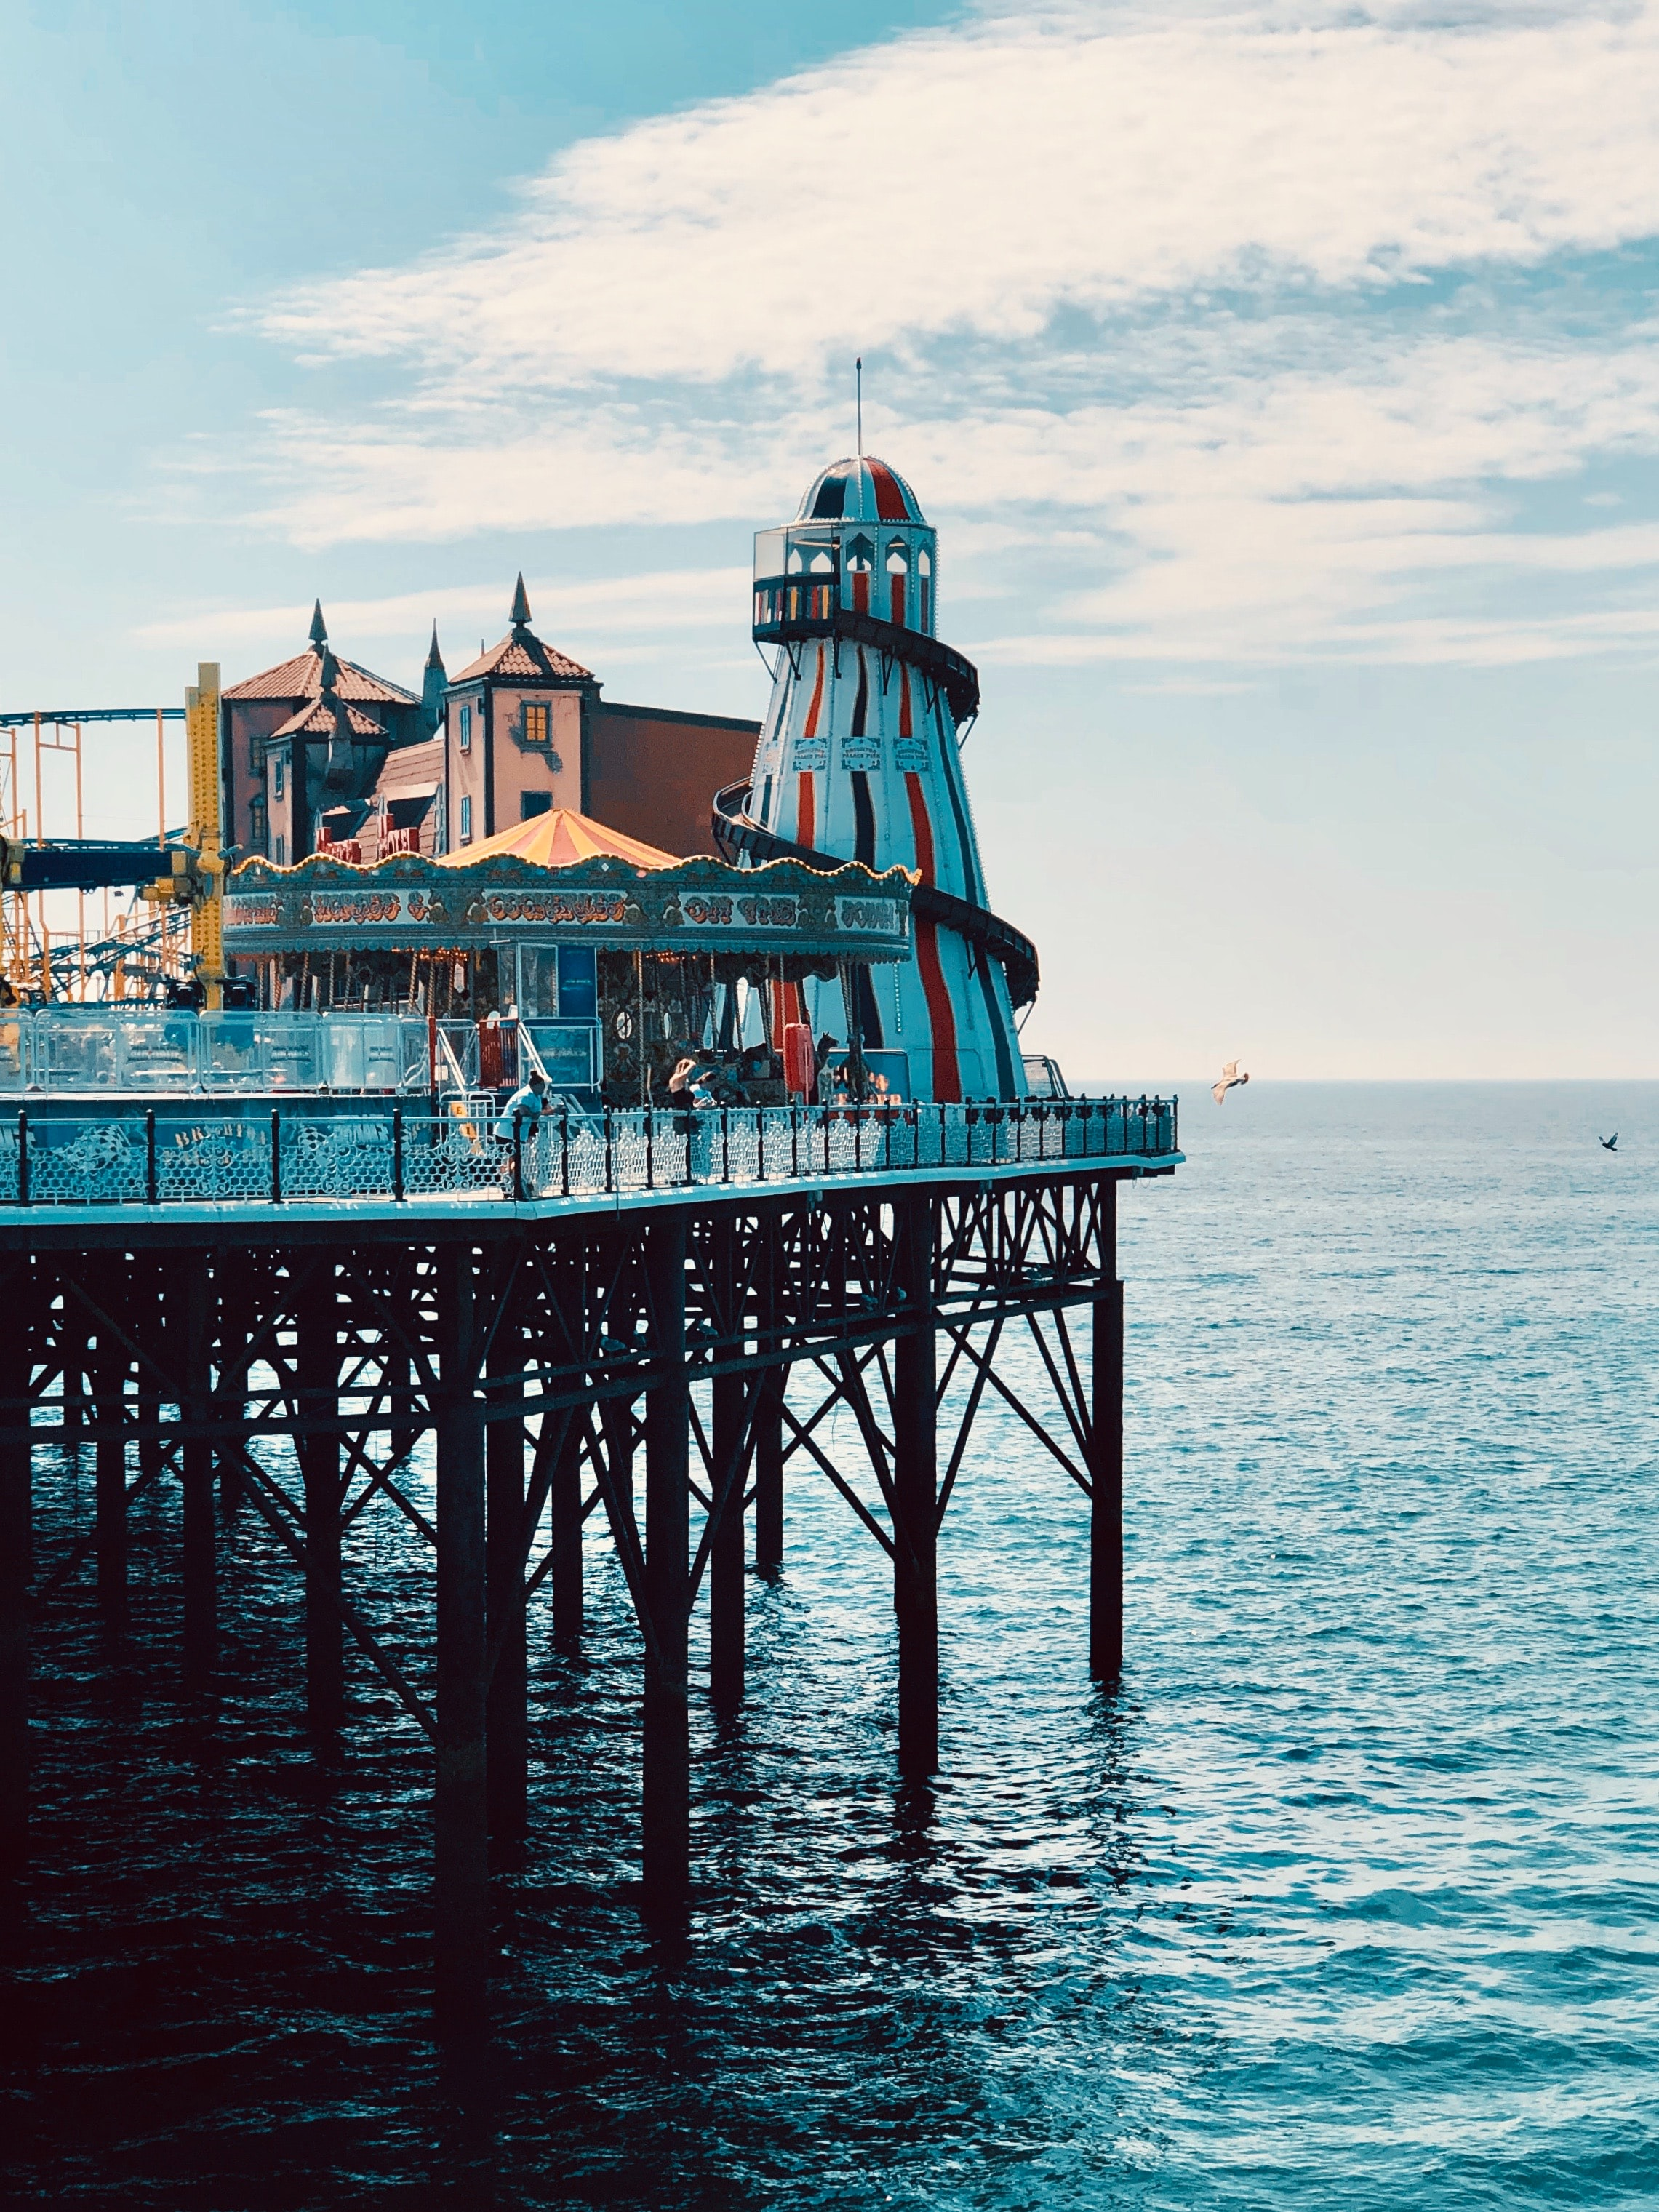
\includegraphics[width=6cm]{src/figures/brighton}}\label{figsupp:sf1}
    \figsupp{This is another supplementary figure.}{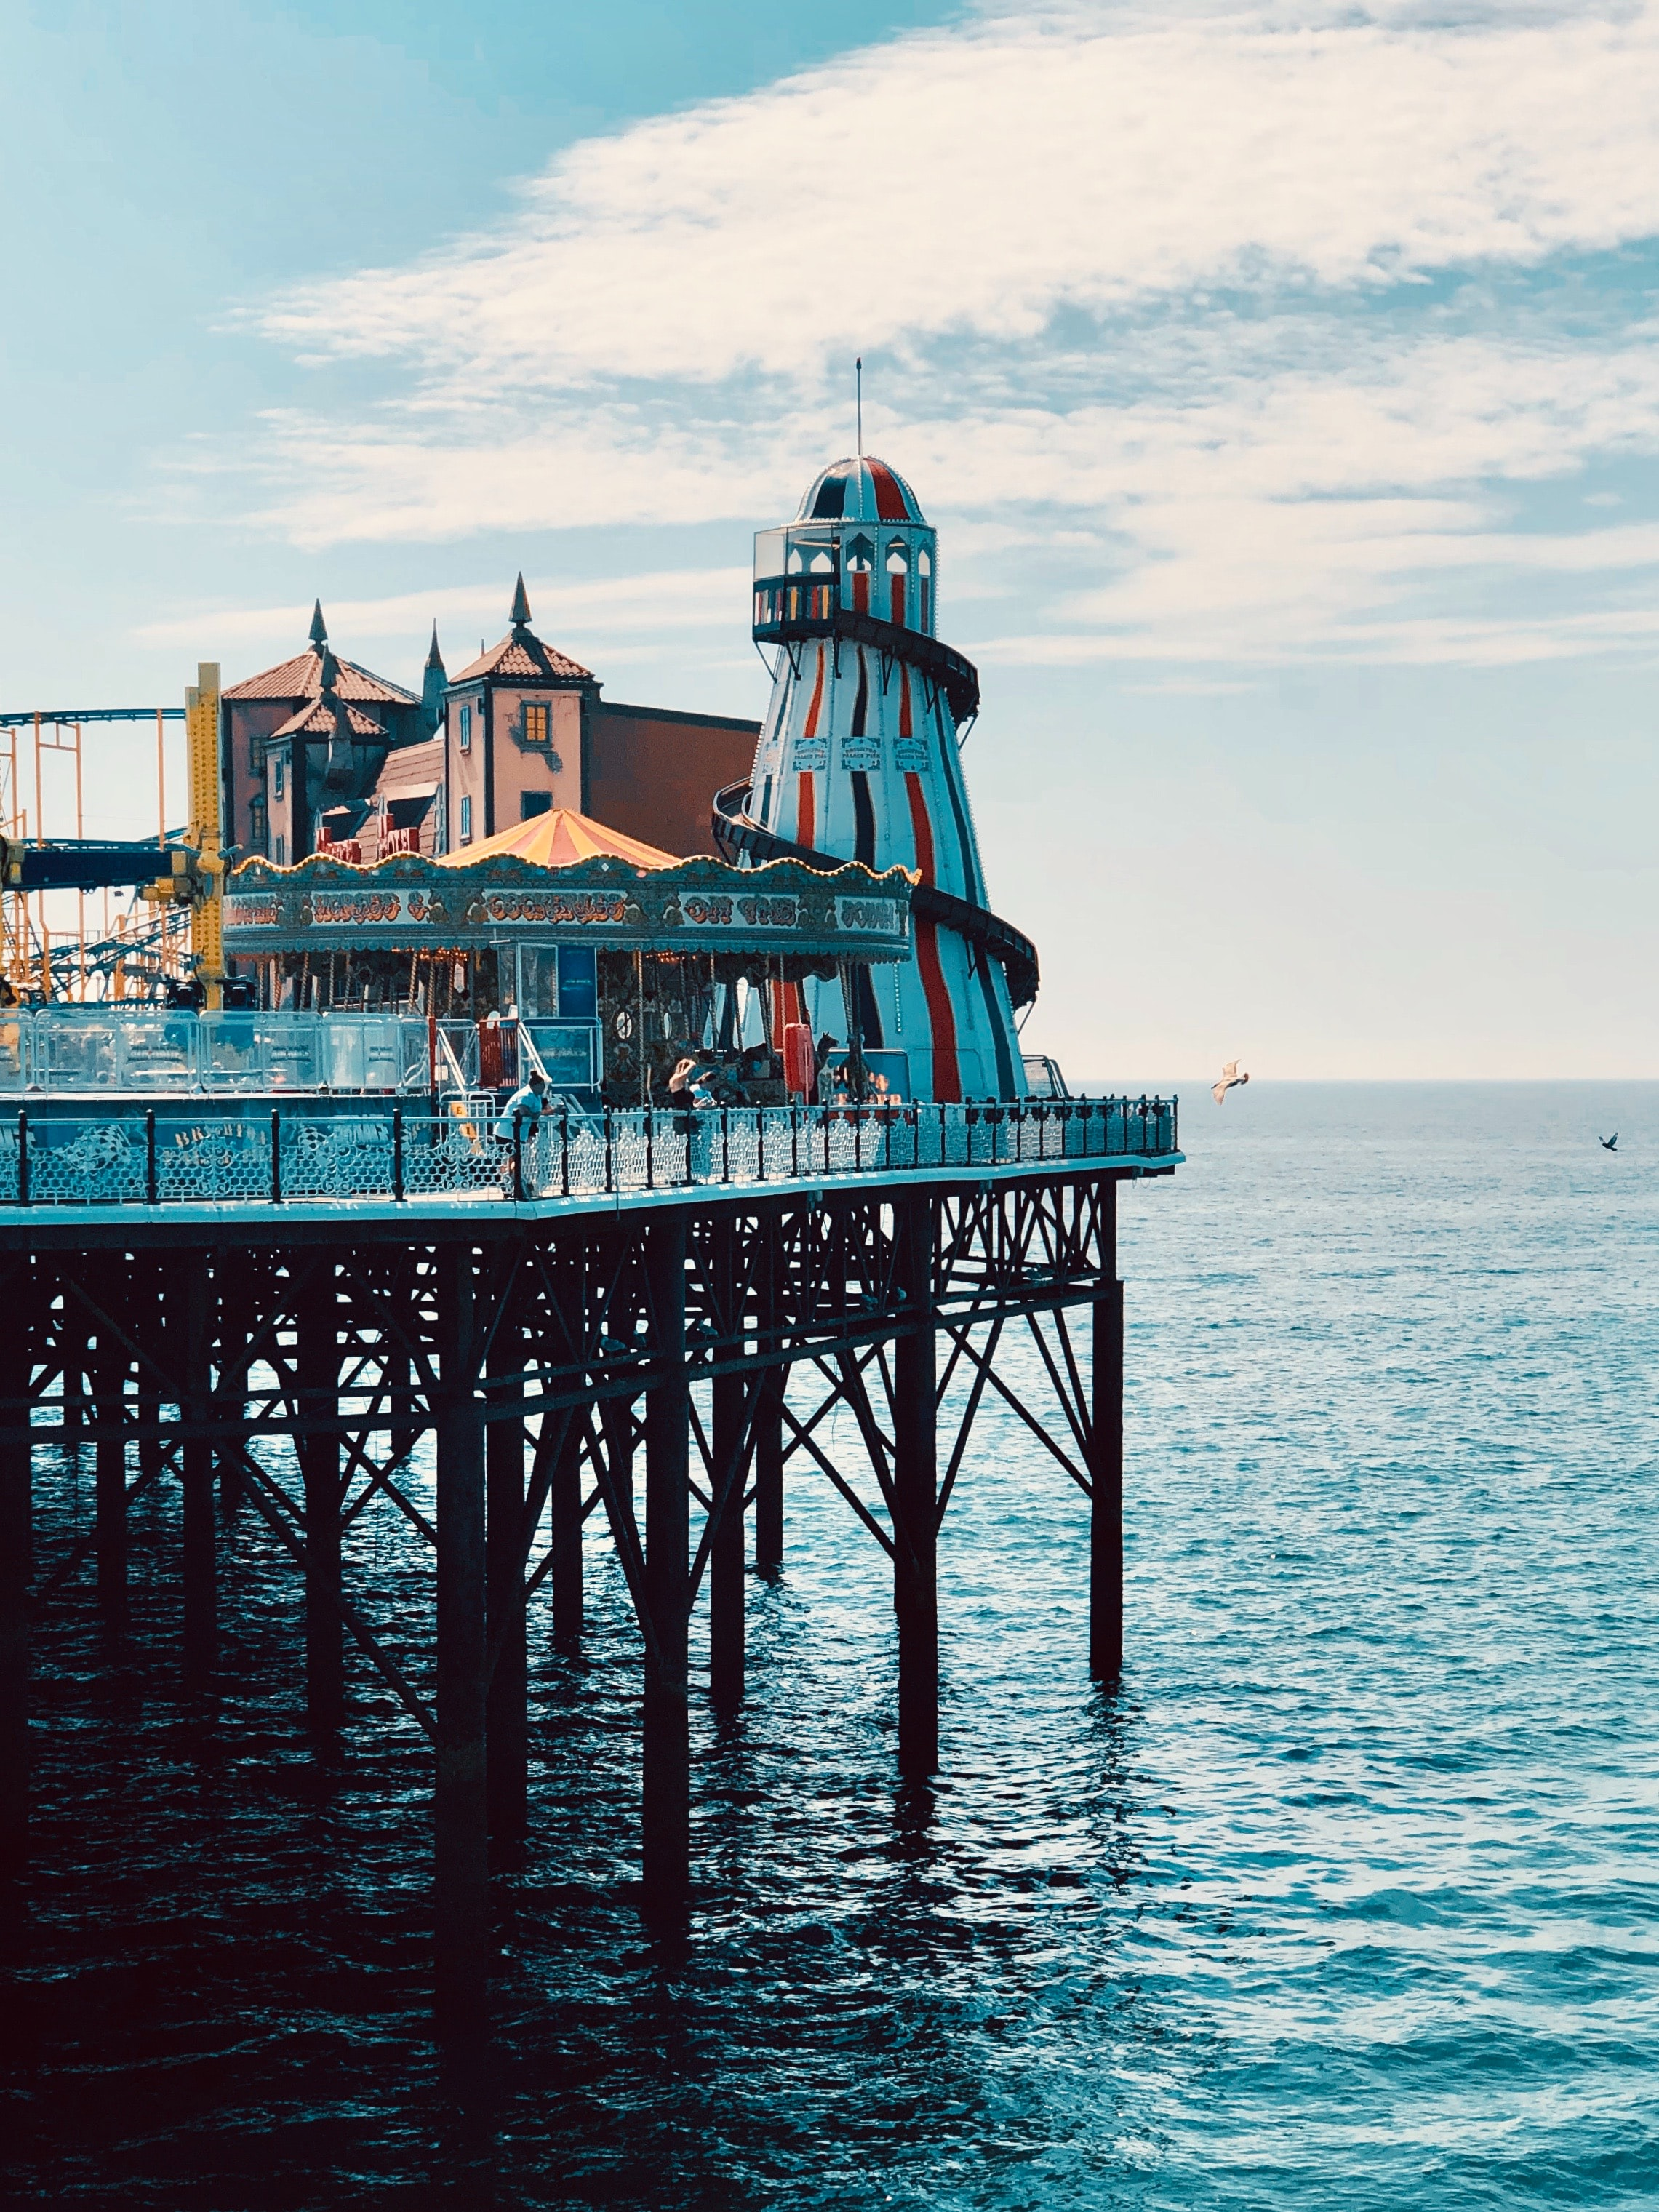
\includegraphics[width=6cm]{src/figures/brighton}}
    \videosupp{This is a description of a video supplement.}\label{videosupp:sv1}
    \figdata{This is a description of a data source.}\label{figdata:first}
    \figdata{This is another description of a data source.}\label{figdata:second}
    \figsrccode{This is a description of a source code.}\label{figsrccode:first}
\end{figure}

\subsection{Other Chemistry Niceties}

You can use commands from the \texttt{mhchem} and \texttt{siunitx} packages. For example: \ce{C32H64NO7S}; \SI{5}{\micro\metre}; \SI{30}{\degreeCelsius}; \SI{5e-17}{\Molar}

\subsection{Lists}

You can make lists with automatic numbering \dots

\begin{enumerate}
    \item Like this,
    \item and like this.
\end{enumerate}
\dots or bullet points \dots
\begin{itemize} 
    \item Like this,
    \item and like this.
\end{itemize}
\dots or with words and descriptions \dots
\begin{description}
    \item[Word] Definition
    \item[Concept] Explanation
    \item[Idea] Text
\end{description}

Some filler text, because empty templates look really poorly. \lipsum[1]
\section{Methods \& Materials} \label{methods}

\subsection{Behavioural setup}
\lipsum[2]

\subsection{Electrophysiological setup}
\lipsum[2] 




\section{Results} \label{results}
\lipsum[1-4]
\input{src/tables/simple-table.tex}
\section{Discussion} \label{discussion}
\lipsum[1-3]
\subsection{Acknowledgment}
This preprint was created using the LaPreprint template (\url{https://github.com/roaldarbol/lapreprint}) by Mikkel Roald-Arb\o l \textsuperscript{\orcidlink{0000-0002-9998-0058}}.

\subsection{Author contributions}
Consider using a contribution table for clarity. I may add it later.
Conceptualization: E.S., B.H.; Methodology: B.H.; Software: B.H.; Validation: S.R.; Formal analysis: S.R.; Investigation: E.S.; Resources: B.H.; Writing - original draft: E.S.; Writing - review \& editing: S.R., B.H.; Visualization: S.R.; Supervision: B.H.; Project administration: B.H.; Funding acquisition: B.H.
% According to https://journals.biologists.com/jeb/pages/author-contributions

\subsection{Supplementary}
Insert the supplementary text here.

\printbibliography

% DON'T EDIT. If "endfloat" option is enabled all floats appear before appendices
\if@endfloat\clearpage\processdelayedfloats\clearpage\fi 


%%%%%%%%%%%%%%%%%%%%%%%%%%%%%%%%%%%%%%%%%%%%%%%%%%%%%%%%%%%%
%%% SUPPLEMENTARY MATERIAL / APPENDICES
%%%%%%%%%%%%%%%%%%%%%%%%%%%%%%%%%%%%%%%%%%%%%%%%%%%%%%%%%%%%
%% Sadly, we can't use floats in the appendix boxes. So they don't "float", but use \captionof{figure}{...} and \captionof{table}{...} to get them properly caption.
\begin{appendix}

\begin{appendixbox}\label{app:ttt}
    \begin{appendixbox}

\end{appendixbox}

\end{appendixbox}

\begin{appendixbox}
    \section{Key resources}

% Make your own table style https://tex.stackexchange.com/questions/94799/how-do-i-color-table-columns
\newcolumntype{A}{p{0.25\textwidth}}
\newcolumntype{B}{p{0.4\textwidth}}
\newcolumntype{C}{p{0.2\textwidth}}
\rowcolors{2}{lightColour!5}{lightColour!5}
\begingroup\footnotesize
\begin{longtable}[l]{|A|B|A|}
    \caption{} \label{tab:resources} \\
    \hline
    \rowcolor{LightGrey!50}
    REAGENT or RESOURCE & SOURCE & IDENTIFIER \\
    \hline
    \rowcolor{white}
    \multicolumn{3}{|l|}{Deposited data} \\
    \hline
    & & \\
    \hline
    \rowcolor{white}
    \multicolumn{3}{|l|}{Experimental models: Organisms/strains} \\
    \hline
    Ground beetle & Stanmer Park, Sussex, UK & \textit{Nebria brevicollis} \\
    \hline
    \rowcolor{white}
    \multicolumn{3}{|l|}{Software} \\
    \hline
    Python & Python & 3.7-3.10 \\
    BuxRecorder & Github ref & v0.1 \\
    OpenSCAD & & \\
    PrusaSlicer & Prusa & \\
    uEye64 & IDS Imaging Development Systems GmbH & \\
    Excel 2010 & Microsoft, Redmond, USA & \\
    R & R Foundation for Statistical Computing, Vienna, Austria & v3.5.1 \\
    RStudio & RStudio Inc, Boston, USA & v1.1.463 \\
    sleeprex & Github repo & v0.1 \\
    sleeprex-analysis & Github repo & v0.1 \\
    \hline
    \rowcolor{white}
    \multicolumn{3}{|l|}{Other} \\
    \hline
    Incubator & & \\
    Pinkies & & \\
    6-well plate & & \\
    Infrared camera & & \\
    Infrared light source & & \\
    Lamp & & \\
    Diffusive fabric & & \\
    Raspberry Pi 4 & & \\
    Breakout garden & & \\
    Light sensor & & \\
    Temperature and humidity sensor & & \\
    Makerbeam & & \\
    3D printer, Prusa Mini+ & & \\


    \hline
\end{longtable}
\endgroup
\end{appendixbox}

\end{appendix}


%%%%%%%%%%%%%%%%%%%%%%%%%%%%%%%%%%%%%%%%%%%%%%%%%%%%%%%%%%%%
%%% ARTICLE END
%%%%%%%%%%%%%%%%%%%%%%%%%%%%%%%%%%%%%%%%%%%%%%%%%%%%%%%%%%%%

\end{document}
